\documentclass[11pt]{scrartcl}

\usepackage{ gensymb }
\usepackage{placeins}
\usepackage{graphicx}
\usepackage{amsmath}

\begin{document}

\title{ELEC2520      Energy System and Control}
\subtitle{LAB REPORT:  Transformer Measurements and Analysis}
\maketitle

\begin{center}
\begin{tabular}{|c|c|}
\hline
Student Name & Student ID \\
\hline
Yingjie Luan & 200829024 \\
\hline
\end{tabular}
\end{center}

\textit{High quality report which deserves good marks is the one that has legible writing, well-sorted equations which show clearly your calculations and well-presented diagrams with clear labels. If additional space is needed, please attach separate sheet(s). It is recommended that this report is typed out and diagrams are computer generated. As only soft-copy submission is allowed, hand-drawn diagrams and hand-written reports must be scanned and included in this document. Nevertheless, they are only accepted if diagrams are in good quality and the texts are still legible. You may complete this report in your own time and submit it through VLE by 11:59pm Friday Week 11. }

\section*{PART 1:  Transformer Open Circuit and Short Circuit Tests}

Write down your results from the Open Circuit and Short Circuit tests in the following table:\\

\begin{tabular}{|c|c|c|c|c|}
\hline
Tests&\multicolumn{2}{c}{Voltage}& Current&Power\\
\hline
Open Circuit& $V_{1oc}=230V$ & $V_{2oc}=117.2V$ & $I_{1oc}=0.25A$&$40W$\\
\hline
Short Circuit&\multicolumn{2}{c}{$V_{1sc}=10.6V$}&$I_{1sc}=3.33A$&$P_{1sc}=32W$\\
\hline
\end{tabular}


\section*{PART 2:  Derivation of Transformer Circuit Parameters and Turns Ratio}

Referring to the approximate equivalent circuit shown in Figure 1 of Lab Instructions, present succinctly  your calculation for Rc, Xm, R and Xl  from the measured results shown in the table of Part 1. Calculate also the transformer turns ratio. (Present the calculation in the remaining space on this page.)\\

We adopted a so called \textit{simplification version of the Equivalent Circuit}. Where we neglect the voltage drop across $R_1$ and $X_{1l}$ on the value of $I_0$ and we also neglect the voltage drop due to $I_0$ flow through $R_c$ and $X_m$.\\
 
\FloatBarrier
Thus we got the following equivalent circuit:
\begin{figure}[h!]
\centering
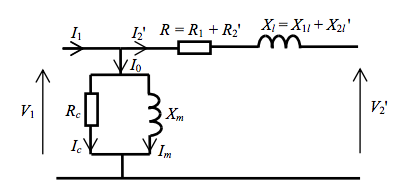
\includegraphics[scale=0.8]{circuit.png}
\caption{Simplified Equivalent Circuit}
\label{img:S_circuit}
\end{figure}
\FloatBarrier

Conduction:\\
\begin{enumerate}
\item While we are doing the open circuit test. There is no voltage drop across $R$ and $X_l$.

Thus we can get the following formula:\\
\begin{equation}
R_c = \frac{V^2_{1oc}}{P_{1oc}}
\end{equation}
\begin{equation}
X_m = \frac{V_{1oc}}{\sqrt{I_{1oc}^2-\left( \frac{V_{1oc}}{R_c}\right)^2}}\end{equation}
\item While we are doing the short circuit test, we neglect the voltage drop across $R_c$ and $X_m$.
Thus we get:\\
\begin{equation}
R = \frac{P_{1sc}}{I_{1sc}^2}
\end{equation}
\begin{equation}
\sqrt{\left(\frac{V_{1sc}}{I_{1sc}}\right)^2-R^2}
\end{equation}

\item What's more, because $V_{2oc}$ is measured, we can get $m = \frac{N_1}{N_2} = \frac{V_{1oc}}{V_{2oc}}$. This indeed is more accurate than the labeled value, which is 2.
\end{enumerate}

Putting in the experiment data we got from the lab, we can get the following values:
\begin{center}
\begin{tabular}{|c|c|}
\hline
Parameters & Values\\
\hline
R & $2.89 \ohm$\\
$X_l$ & $1.33\ohm$\\
$R_c$ & $1322.5\ohm$\\
$X_m$ & $1280.66 \ohm$\\
$\frac{N_1}{N_2}$ & 1.96\\
\hline
\end{tabular}
\end{center}
%\footnote{Figure\ref{img:S_circuit} is from the lab manual}

\section*{PART 3 – Analysis of a Transformer’s Operation with Load}

\subsection*{i Referring to the approximate equivalent circuit shown in Figure 1 of Lab Instructions, draw the phasor diagram relating the voltage V2', current I2', phase angle φ2, voltage drops I2'R and I2'Xl, voltage V1, currents Ic, Im and I1. (Use the phasor V2' as reference along vertical axis. Indicate clearly the phase angles φ1 and φ2.  All phasors must be clearly labelled.)}

\FloatBarrier
The related parser diagram,
\begin{figure}[h!]
\centering
\includegraphics[scale=0.2]{parser.png}
\caption{The parser diagram}
\end{figure}
\FloatBarrier




\subsection*{ii)   Given that the iron (core) losses can be neglected, calculate the primary voltage (V1), current (I1) and the power factor (cos φ1) of the tested transformer when it is supplying 110 V and 3 A to a load with power factor cosφ2 = 0.866 lagging. In the calculations, refer the secondary voltage (110 V) and current (3 A) to the primary side and use the phasor V2' as the reference. Show your calculation succinctly (max one page).}

\FloatBarrier
Referring from this circuit and the related electrical parameter notations,
\begin{figure}[h!]
\centering
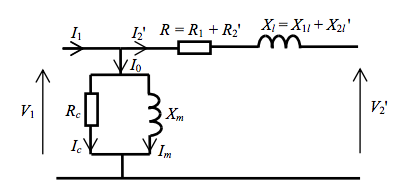
\includegraphics[scale=0.8]{circuit.png}
\caption{Simplified Equivalent Circuit}
\label{img:cal}
\end{figure}
\FloatBarrier
Please notice that the angle is expressed in the unit of radian in following calculation.\\

Let the $ratio = m = 1.96$, thus:\\

$V_2' = V_2 * m = 215.6 V$, $I_2' = I_2/ m= 1.531$.\\

 what's more, $\cos(\varphi) = 0.86$ and the current is lagging, we can see $ \varphi = \arccos(0.86) = -0.5355$.\\
 
To calculate the $V_1$:
\begin{eqnarray*}
V_1 &=& V_2' + I_2' *(R + X_l)\\
 &=& 215.6 + 1.531*e^{-j*0.5355}*(2.89+1.33j)\\
 &=&220.444-0.507j\\
 &=&220.445*e^{-0.0023j}
\end{eqnarray*}

To calculate the $I_0$:
\begin{eqnarray*}
I_0 &=& \frac{V_1}{\frac{1}{\frac{1}{R_c}+\frac{1}{X_m}}}\\
&=& 0.165 - 0.173j
\end{eqnarray*}

To calculate the $I_1$:
\begin{eqnarray*}
I_1 &=& I_O + I_2'\\
&=& 1.482 - 0.954j\\
&=& 1.762*e^{-0.572j}
\end{eqnarray*}

$\varphi_1$ is the angle between the $V_1$ and $I_1$, we can get:
\begin{eqnarray*}
z &=& \frac{V_1}{I_1}\\
&=& 105.349+67.468j\\
&=& 125.101*e^{0.570}
\end{eqnarray*}
Thus, $\varphi_1 = 0.570$, $\cos(\varphi_1) = 0.842$


\footnote{Figure\ref{img:S_circuit} and Figure \ref{img:cal} is from the lab manual}
\end{document}
